\documentclass[
	classe=$1^{ere}STI2D$,
	headerTitle=Informatique
]{exercice}

\usepackage{tcolorbox}
\usetikzlibrary{calc}

\title{Séance informatique : fonctions et tableur}

\begin{document}

\maketitle

\section{Optimiser ses recettes}

\begin{tcolorbox}
	Une entreprise artisanale fabrique des chaises de salon. Elle peut en fabriquer au maximum 25 par jour. Le coût de fabrication de $x$ chaises est donné par la fonction $C$ ci-dessous :
	$$ C(x) = 0,2x³ - 5,05x² + 48,6x + 13,8 $$

	La recette de la vente de ces $x$ chaises est modélisée par la fonction $R$ ci-dessous :
	$$ R(x) = 40x - 0,05x² $$
\end{tcolorbox}


On veut réaliser la feuille de calculs suivante :

\begin{center}
	\includegraphics[width=0.5\linewidth]{Activité - tableur (image 1).png}
\end{center}

\begin{enumerate}
	\item Préparer la feuille de calcul ci-dessus pour une quantité variant de 0 à 25 chaises.

	      Entrer une formule dans les cellules B2 et C2, et l'étirer vers le bas afin de compléter automatiquement les colonnes B et C.
	\item \begin{enumerate}
		      \item Sélectionner les colonnes A, B et C, et insérer un diagramme pour représenter les courbes représentative des fonctions $C$ et $R$.

		            \begin{center}
			            \tipbox{Aide :

				            Utiliser le diagramme XY (dispersion)}
		            \end{center}
		      \item Déterminer graphiquement le nombre de chaises produites et vendues pour que l'entreprise réalise un bénéfice.
		      \item Déterminer graphiquement la quantité de chaises à produire et à vendre pour réaliser un bénéfice maximum. Avec la précision permise par le graphique, donner approximativement ce bénéfice maximum.
	      \end{enumerate}
	\item \begin{enumerate}
		      \item Pour vérifier les résultats de la question précédente, ajouter une colonne \textit{Bénéfice} dans la colonne D. Quelle formule peut-on utiliser en D2 qui, une fois étirée vers le bas, permet d'automatiser les calculs de la colonne D ?
		      \item Retrouver alors le bénéfice maximal espéré. Pour quelle quantité de chaises produites ce bénéfice est-il réalisé ?
	      \end{enumerate}
\end{enumerate}

\section{Optimisation du volume d'une boîte}

\begin{tcolorbox}
	On veut, à partir d'une feuille de papier cartonné de format $21$ cm $×$ $29,7$ cm, créer une boîte rectangulaire de volume maximum.

	Pour ce faire, on découpe dans chaque coin des carrés de côté $x$ cm.

	\begin{center}
		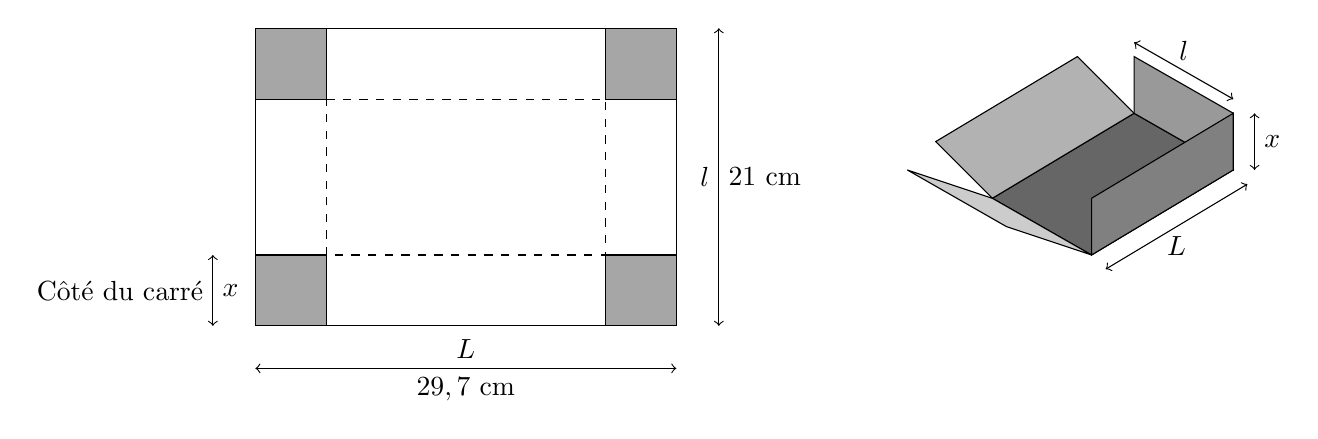
\begin{tikzpicture}[scale=0.18]
			\newcommand{\longueurX}{5}
			\draw (0,0) -- ++(29.7,0) -- ++(0,-21) -- ++(-29.7,0) -- cycle;
			\draw[fill=gray!70] (0,0) -- ++(\longueurX,0) -- ++(0,-\longueurX) -- ++(-\longueurX,0) -- cycle;
			\draw[fill=gray!70] (0,-21) -- ++(\longueurX,0) -- ++(0,\longueurX) -- ++(-\longueurX,0) -- cycle;
			\draw[fill=gray!70] (29.7,0) -- ++(-\longueurX,0) -- ++(0,-\longueurX) -- ++(\longueurX,0) -- cycle;
			\draw[fill=gray!70] (29.7,-21) -- ++(-\longueurX,0) -- ++(0,\longueurX) -- ++(\longueurX,0) -- cycle;
			\draw[dashed] (\longueurX,-\longueurX) -- ++(29.7-2*\longueurX,0) -- ++(0,-21+2*\longueurX) -- ++(-29.7+2*\longueurX,0) -- cycle;
			\draw[<->] (0,-21) ++(-3,0) -- node[right] {$x$} node[left] {Côté du carré} ++(0,\longueurX);
			\draw[<->] (0,-21) ++(0,-3) -- node[above] {$L$} node[below] {$29,7$ cm} ++(29.7,0);
			\draw[<->] (29.7,-21) ++(3,0) -- node[left] {$l$} node[right] {$21$ cm} ++(0,21);

			\coordinate (Boite) at (52,-12);
			\renewcommand{\longueurX}{4}
			\coordinate (Longueurl) at (7,-4);
			\coordinate (LongueurlRev) at (-7,4);
			\coordinate (LongueurL) at (10,6);

			\draw[fill=black!60] (Boite) -- ++(Longueurl) -- ++(LongueurL) -- ++(LongueurlRev) -- cycle;
			\draw[fill=black!30] (Boite) -- ++(-\longueurX,\longueurX) -- ++(LongueurL) -- ++(\longueurX,-\longueurX) -- cycle;
			\draw[fill=black!20] (Boite) -- ++(-6,2) -- ++(Longueurl) -- ++(6,-2) -- cycle;
			\draw[fill=black!40] (Boite) ++(LongueurL) -- ++(0,\longueurX) -- ++(Longueurl) -- ++(0,-\longueurX) -- cycle;
			\draw[fill=black!50] (Boite) ++(Longueurl) -- ++(0,\longueurX) -- ++(LongueurL) -- ++(0,-\longueurX) -- cycle;

			\draw[<->] (Boite) ++($(Longueurl) + (1,-1)$) -- node[below] {$L$} ++(LongueurL);
			\draw[<->] (Boite) ++($(LongueurL) + (0,\longueurX + 1)$) -- node[above] {$l$} ++(Longueurl);
			\draw[<->] (Boite) ++($(Longueurl) + (LongueurL) + (1.5,0)$) -- node[right] {$x$} ++(0,\longueurX);
		\end{tikzpicture}
	\end{center}

	On se demande alors : quelle est la valeur de $x$ pour laquelle le volume de la boîte est maximal ?
\end{tcolorbox}

\begin{enumerate}
	\item Justifier que $x$ est un nombre réel dans l'intervalle $\intervalle{[}{0}{10,5}{]}$.
	\item Entrer une formule dans les cellules B2, C2 et D2, et l'étirer vers le bas afin de compléter automatiquement les colonnes B, C et D.

	      \begin{center}
		      \includegraphics[width=0.5\linewidth]{Activité - tableur (image 2).png}
	      \end{center}
	\item Quel semble alors être le volume maximal de la boîte ?

	      Pour quelle valeur de $x$ ?
\end{enumerate}

\end{document}